\section{Expected System Diagram}
\begin{figure}[!ht]
    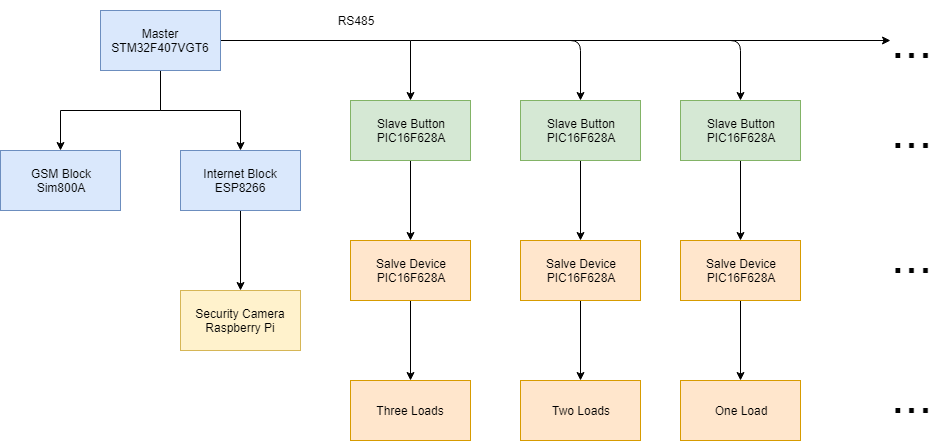
\includegraphics[scale=0.5]{images/hardwareBlock.png}
    \caption{Expected hardware blocks}
    \label{fig:hardwareBlock}
\end{figure}

    \begin{table}[h!]
    \begin{center}
    \begin{tabular}{ |c|c|c|  }
      \hline
      Attributes & Detail & Notes\\
      \hline
      Maximum number of devices&   99& Can be extended by\\
      & &extending command frame\\
      \hline
      Longest distance supported&   1200 meters&\\
      \hline
      Communication method &Mainly RS-485&\\
      \hline
      Wi-Fi connection & Wi-fi 2.4GHz&\\
      \hline
     \end{tabular}
     \caption{System ideal characteristics}
     \label{table:idealCharacteristics}
    \end{center}
    \end{table}
    In Figure~\ref{fig:hardwareBlock}, there are blocks named Master, Slave Buttons, Slave Devices, GSM block, Internet block and Security Camera. Each block is indicated with implemented hardware and how they connect to each other. As in the figure~\ref{fig:hardwareBlock}, Master is connecting with number of Slaves by UART over RS-485; Also, Master is implemented with GSM and Internet blocks in order to help end user controlling devices and receiving alerts over GSM or Wi-Fi. Each slave connects to the system has the same working principle but different names. In this thesis, there are two slave-2-devices and one slave-3-devices alongside with two slave-2-buttons and one slave-3-buttons to control the loads, respectively. Besides, the author designed one slave-2-buttons and one slave-1-button to control three out of seven existed devices. Three slave-devices are implemented with relays switch state for devices in the house, last device (Device 3) of slave-3-devices is assigned as the Main Door trigger to demonstrate the Security Camera System with Facial Recognition later on.

    Internet Block is the middle man for communicating between Web Server and the System. With this block implemented, end-user can control devices without pushing the physical buttons, which may causes difficulties for users because the owners can control their house whenever and wherever they want. Besides, with the help of the Web Server, end-users can collect and monitor data in the house in order to diagnostic and maintain precisely. GSM block should be installed in order to help in the event that Internet block is having unexpected problems.

    Security Camera block is the block that monitors the main door and inside the house. The camera installed outdoor is responsible for outdoor security in which it will track people entering the house with a facial recognition system. Additionally, indoor camera should handle the motion detection system while the owner is not at home in order to find strange motion which maybe a burglar breaking in the house. These two system will track and alert by emails, mobile application and text message over GSM network in the case that they detect something. Furthermore, the three-dots indicates that the system can be extended with number of slaves over RS-485, but only up to 99 dues to the limitation of command frame.
%Master hardware design
\section{Master Design}\label{masterDesign}
    \subsection{Microcontroller Requirements}
    There are few requirements for the Microcontroller that the author decided to build the system for the thesis, listed as following.
    \begin{itemize}
        \item Support UART in order to communicate with other modules, namely RS-485, and ESP8266.
        \item Has widely support community.
        \item Easy to learn to program.
        \item Extendable with installed components.
        \item Price and ability for effortless replacement.
      \end{itemize}
      \begin{figure}[!ht]
        \begin{center}
        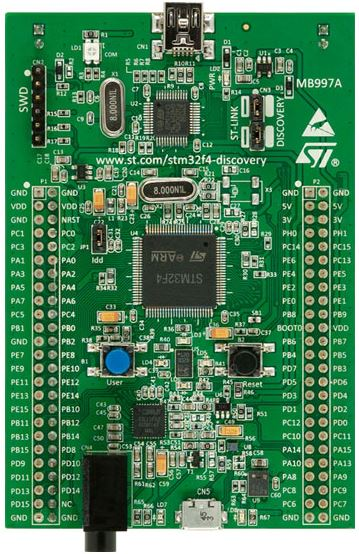
\includegraphics[scale=1]{images/stm32f4_discovery.jpg}
        \caption{STM32F4 Discovery Kit}
        \label{fig:stm32Kit}
        \end{center}
      \end{figure}
      Based on the requirements, the chosen MCU is STM32F407VGT6 with STM32F4 Discovery Kit from STMicroelectronics. Figure~\ref{fig:stm32Kit} refers the real kit in the market. It is considered as a suitable MCU because of the following reasons.
      \begin{itemize}
        \item The board has large support community.
        \item Programmed with C language with countless documents.
        \item MCU used is STM32F407VGT6, with core ARM Cortex 32bit M4, clock up to 168Mhz.
        \item Support up to 140 I/O.
        \item Flash memory 1MB.
        \item Easy to flash even with end-user.
        \item Cheap price and easy to find replacement parts.
      \end{itemize}
      \begin{figure}[!ht]
        \begin{center}
        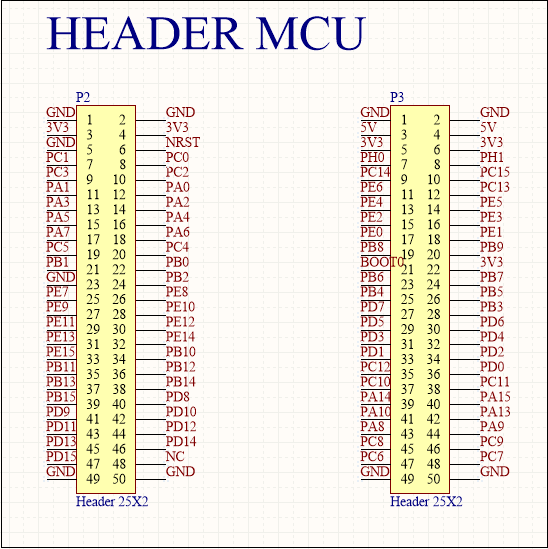
\includegraphics{images/headerMcu.PNG}
        \caption{Header for STM32F4 Discovery Kit}
        \label{fig:headerMcu}
        \end{center}
      \end{figure}
      In this thesis, to ensure the effortless replacement of the system parts, the author designed with modules attached on PCB by using headers. With this method, whenever an error occurs to any part of the system, end-user can replace the broken part easily without replacing the whole system. Figure~\ref{fig:headerMcu} shows the headers on Master board for STM32F4 Discovery Kit which is chosen for the thesis. In addition, it shows the connection pin of the MCU with other modules over UART. To be more specific, MCU connects with RS-485 module over UART1 via pin PB6-PB7, with module ESP8266 over UART2 via pin PD5-PD6, with module SIM800A over UART3 via pin PD8-PD9.
      %hardware RS-485
      \subsection{Module RS-485}
      \begin{figure}[!ht]
        \begin{center}
        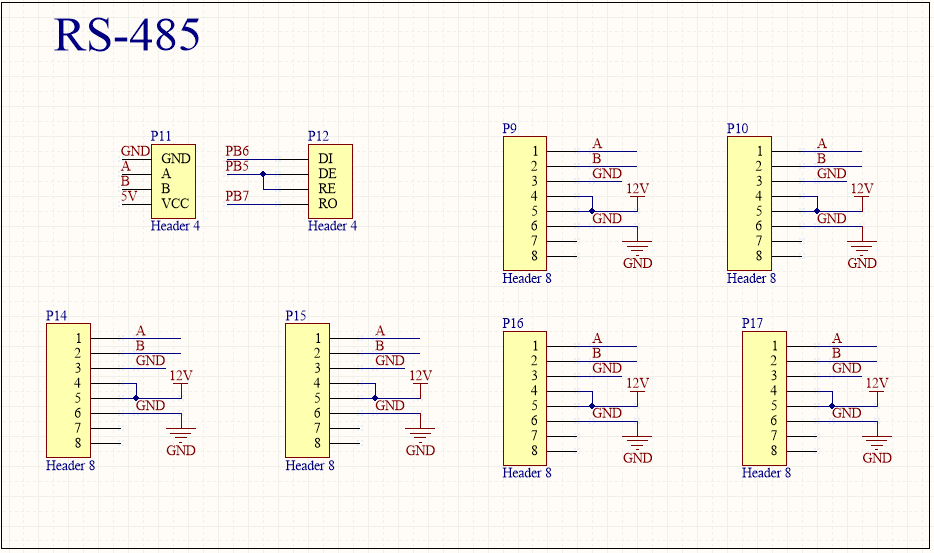
\includegraphics[scale=0.63]{images/header485.PNG}
        \caption{Header for module RS-485}
        \label{fig:header485}
        \end{center}
      \end{figure}
      \begin{figure}[!ht]
        \begin{center}
        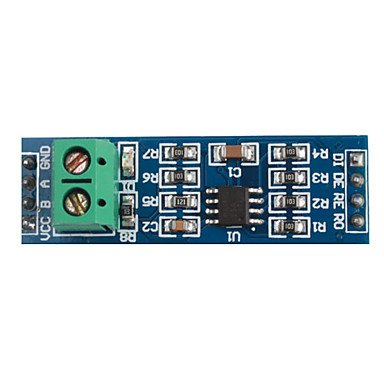
\includegraphics[scale=1]{images/module-rs485.png}
        \caption{Module RS-485}
        \label{fig:module485}
        \end{center}
      \end{figure}

      Figure~\ref{fig:module485} refers the cheap version of module TTL to RS-485 on the market. It integrated IC MAX485 as the main component and other sub-components included termination resistor. This module is stable enough for the system and easy to replace due to its cheap price but does has a weakness which is if it is broken, end-user cannot know unless further tests on the module is processed. The table~\ref{table:module485PinOut} indicates the pin out guideline to connect with the MCU. According to datasheet of IC MAX485, RE and DE must be connected for the MCU to control the module based on logic level, in which the module is transmitting if the pins are pull up to 1, otherwise it is receiving.
      \begin{table}[h!]
        \begin{center}
        \begin{tabular}{ |c|c|  }
          \hline
          Pin & Detail\\
          \hline
          VCC& 5V\\
          \hline
          A&   Non-inverting Receiver Input and Non-inverting Driver Output\\
          \hline
          B &.Inverting Receiver Input and Inverting Driver Output\\
          \hline
          GND & GND, should be 0V\\
          \hline
          RO & Receiver Output (to Rx pin of microcontroller)\\
          \hline
          RE & Receiver Output Enable (Low to enable)\\
          \hline
          DE & Driver Output Enable (high to enable)\\
          \hline
          DI & Driver Input (to Tx pin of microcontroller)\\
          \hline
         \end{tabular}
         \caption{Module UART TTL to RS-485 pin out}
         \label{table:module485PinOut}
        \end{center}
        \end{table}
      
      Figure~\ref{fig:header485} shows the headers which are used on Master board for RS-485 module in figure~\ref{fig:module485} and the headers of RJ-11 female jack for RS-485 output of the Master. The reason for choosing RJ-11 jack and its compatible cable is the cable suits for the project which needs four wires, in which two are the signal wires (A and B of RS-485 standard) and the other two are the pair providing power for other slaves (12V and GND). With this method, a four-wire twisted cable with shield is used in order to keep the noise as low as possible and still, provides the power along the whole system with only one cable connected.

      \subsection{Module ESP-8266}
      This module is implemented to establish the connection between the Web Server and the System. End-users can control and monitor their system with a website or an android application over Wi-Fi connection with module ESP-8266. There are various versions of module using ESP-8266 on the market, but the full name of the chosen module is ESP-8266 NodeMCU lua CP2102. It is a small size kit that integrated with ESP8266 SoC, other components and it is also compatible with Arduino IDE which makes it become the easiest to use ESP-8266 module in comparison to other versions.
      \begin{table}[h!]
        \begin{center}
        \begin{tabular}{ |c|c|  }
          \hline
          Attribute & Detail\\
          \hline
          SoC& ESP8266 Wifi SoC\\
          \hline
          Firmware&   NodeMCU Lua\\
          \hline
          Flash chip &CP2102\\
          \hline
          GPIO & compatible with firmware of Node MCU\\
          \hline
          Power supply & 5V DC with Micro USB or Vin\\
          \hline
          GPIO logic level & 3.3V\\
          \hline
          Integrated LED & Reset, Flash and Status indicator\\
          \hline
          Dimension & 25mm x 50mm\\
          \hline
          Others& Compatible with Arduino IDE\\
          \hline
         \end{tabular}
         \caption{Module ESP-8266 NodeMCU lua CP2102 remarkable characteristics}
         \label{table:moduleEspDetail}
        \end{center}
        \end{table}

        \begin{figure}[!ht]
            \begin{center}
            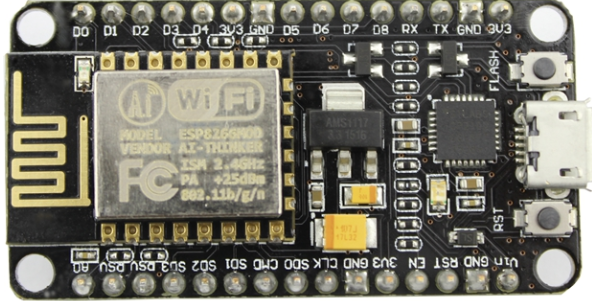
\includegraphics[scale=0.9]{images/module-esp.png}
            \caption{Module ESP-8266 NodeMCU lua CP2102}
            \label{fig:moduleEsp}
            \end{center}
          \end{figure}

          % \subsection{Module SIM800A}

          \subsection{Power for Master}\label{powerForMasterDesign}
          In order to provide enough power for every module mentioned above, the author uses a AC/DC adapter with output 12V-5A as the main power supply with a honeycomb power source 12V-3A as a backup one as illustrated in Figure~\ref{fig:powerMaster}. In the Power for Master circuit, module LM2596 which is a buck converter, used to convert 12VDC to 5VDC. 
          \begin{figure}[!ht]
            \begin{center}
            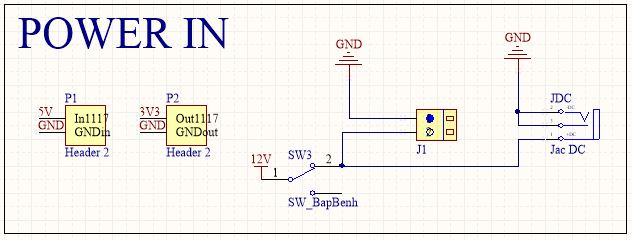
\includegraphics[scale=0.8]{images/powerMaster.JPG}
            \caption{Header for Power blocks for Master}
            \label{fig:powerMaster}
            \end{center}
          \end{figure}
          \begin{figure}[!ht]
            \begin{center}
            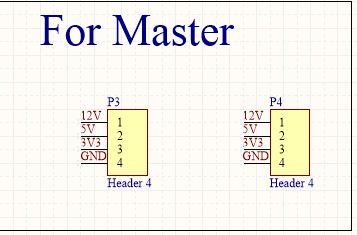
\includegraphics[scale=1]{images/headerPowerOut.JPG}
            \caption{Output header of Power for Master}
            \label{fig:headerPowerOut}
            \end{center}
          \end{figure}
          \begin{figure}[!ht]
            \begin{center}
            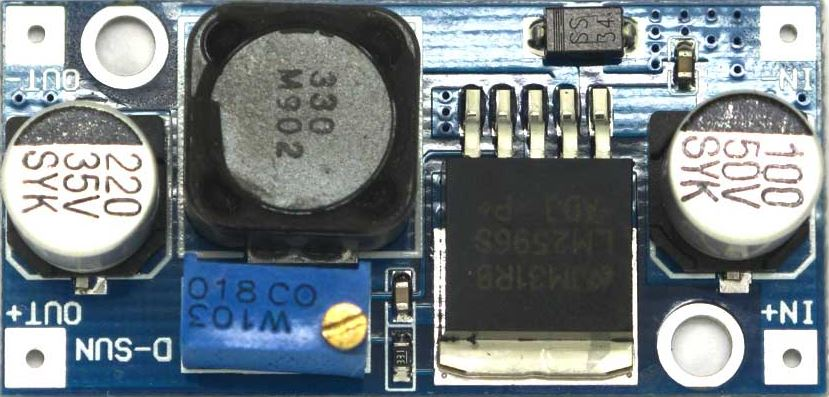
\includegraphics[scale=0.6]{images/module-2596.jpg}
            \caption{Module LM2596}
            \label{fig:module2596}
            \end{center}
          \end{figure}
          \begin{figure}[!ht]
            \begin{center}
            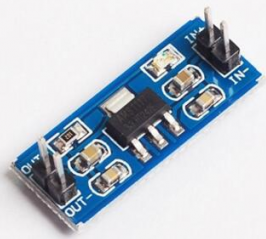
\includegraphics[scale=1]{images/module1117.png}
            \caption{Module ASM1117}
            \label{fig:module1117}
            \end{center}
          \end{figure}

          \begin{table}[h!]
            \begin{center}
            \begin{tabular}{ |c|c|  }
              \hline
              Attribute & Detail\\
              \hline
              Input& Ranging 3V-30V\\
              \hline
              Output&   Ranging 1.5V-30V\\
              \hline
              Maximum current output &3A\\
              \hline
              Efficiency & 92\%\\
              \hline
              Power & 15W\\
              \hline
              Dimension & 45mm x 20mm x 14mm\\
              \hline
             \end{tabular}
             \caption{Module LM2596 specifications}
             \label{table:module2596}
            \end{center}
            \end{table}
            Table~\ref{table:module2596} lists remarkable specifications of module LM2596 using in the project. With these specifications and its cheap price, the module is suitable for various applications, namely voltage dividing, buck converting, supplying for motor, camera or robot.
            In Figure~\ref{fig:powerMaster}, P1 and P2 headers are implemented for module AMS1117. AMS1117 is also a buck converter but from 5VDC to 3.3VDC only. The advantage of this module is that it is integrated in a small circuit (as in Figure~\ref{fig:module1117}) can supply and maintain maximum current from 800mA to 1A, which is needed for modules that need high current such as module ESP-8266 using in this thesis. Furthermore, the 3.3VDC may be used as a backup power supply for Microcontroller which needs 3.3V, which could be extended in further development of the project. Figure~\ref{fig:headerPowerOut} indicates the output headers for circuit Power for Master, which will supply the Master with three level of voltage source, namely 12V, 5V and 3.3V.
            
\section{Slave Design}
    \subsection{Requirements}
    Slave circuits have requirements listed as following.
        \begin{itemize}
        \item Small integrated circuit.
        \item Support UART to communicate with Master.
        \item Well documented.
        \item Large support community.        
        \item Price is cheap.
        \item Easy to implement or replace when broken.
        \end{itemize}
        \begin{figure}[!ht]
            \begin{center}
            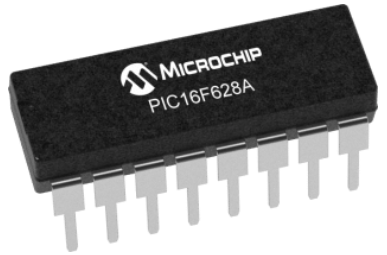
\includegraphics[scale=1]{images/pic16f628a.png}
            \caption{Microchip PIC16F628A}
            \label{fig:picf16f628a}
            \end{center}
        \end{figure}
        The author chose PIC16F628A as the microcontroller for Slave Buttons and Slave Devices because of its small size, easy to implement or replace and reasonable price. Please see Table~\ref{table:pic16f628aSpecs} for the highlight specifications of MCU Microchip PIC16F628A.
        \begin{table}[h!]
            \begin{center}
            \begin{tabular}{ |c|c|  }
              \hline
              Attribute & Detail\\
              \hline
              Supply power& Ranging 2V-5.5V\\
              \hline
              Number of pins&   18\\
              \hline
              RAM &224 bytes\\
              \hline
              EEPROM & 128 bytes\\
              \hline
             \end{tabular}
             \caption{PIC16F628A Highlight Specifications}
             \label{table:pic16f628aSpecs}
            \end{center}
            \end{table}

    \subsection{Power for Slaves}
    In comparison with Master, power supply for Slaves requires less criteria. There are two blocks of power will supply for slaves in this thesis. In the first design, the author built power block separately from the circuit, but in second design, the power supply for the Slaves is integrated in the same circuit in each Slaves. Please see Figure~\ref{fig:powerForSlave1} and Figure~\ref{fig:powerForSlave2} for two blocks that supply power for Slaves in the first and second design, respectively. In first design, power block use the same buck converter LM2596 and ASM1117 as mentioned in section \ref{powerForMasterDesign} Power for Master, but in second design, the author chose IC 7805 for all power blocks using in all later Slaves. First design applied for two slaves, namely Slave-3-Relays and Slave-3-Buttons, the second design implemented on all later Slaves, namely Slave-2-Relays, Slave-2-Buttons and Slave-1-Button.
    \begin{figure}[!ht]
        \begin{center}
        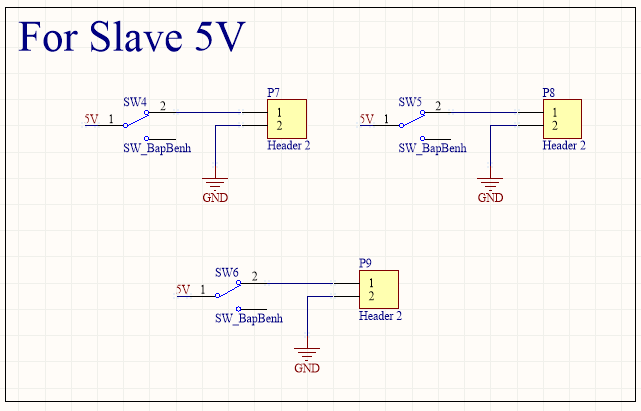
\includegraphics[scale=0.8]{images/powerForSlave1.png}
        \caption{Power supply for Slaves 1}
        \label{fig:powerForSlave1}
        \end{center}
    \end{figure}
    \begin{figure}[!ht]
        \begin{center}
        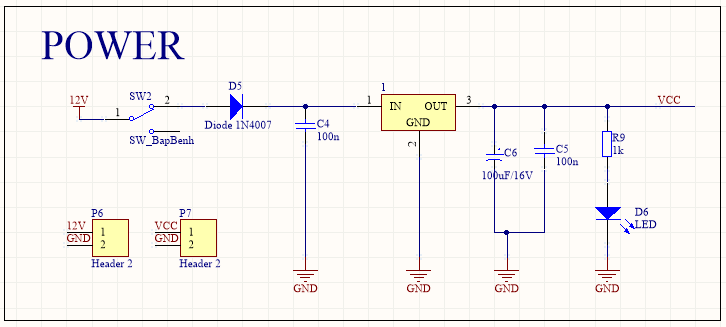
\includegraphics[scale=0.8]{images/powerForSlave2.png}
        \caption{Power supply for Slaves 2}
        \label{fig:powerForSlave2}
        \end{center}
    \end{figure}

    \subsection{Module RS-485}
    Slaves receiving from and transmitting to Master over RS-485 block. In Slave design, the author uses the same module as in Figure~\ref{fig:module485}, the headers for Module RS-485 is also identical to the headers using in Master circuit, but the headers for the output by jack RJ-11 is reduced to two as in the Figure~\ref{fig:header485Slave}.
    \begin{figure}[!ht]
      \begin{center}
      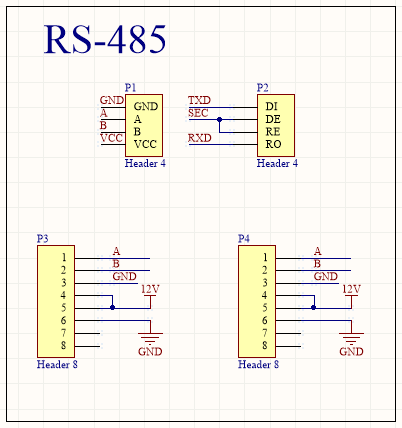
\includegraphics[scale=1]{images/header485Slave.png}
      \caption{Header for module RS-485 in Slave circuits}
      \label{fig:header485Slave}
      \end{center}
  \end{figure}

  \subsection{Controller Block}
  As mentioned in previous section, PIC16F628A is chosen as the MCU for all Slaves in the system. Figure~\ref{fig:mcuButton} and Figure~\ref{fig:mcuRelay} refers the MCU block of Slave Button(s) and Slave Relay(s), respectively, in which connect with external crystal with frequency of 20MHz.
  \begin{figure}[!ht]
    \begin{center}
    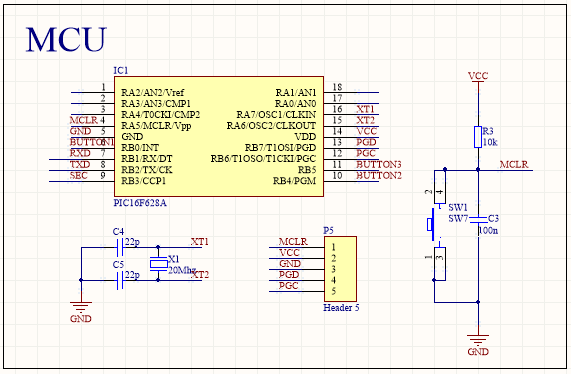
\includegraphics[scale=0.93]{images/mcuButton.png}
    \caption{MCU of Slave Button(s)}
    \label{fig:mcuButton}
    \end{center}
\end{figure}
\begin{figure}[!ht]
    \begin{center}
    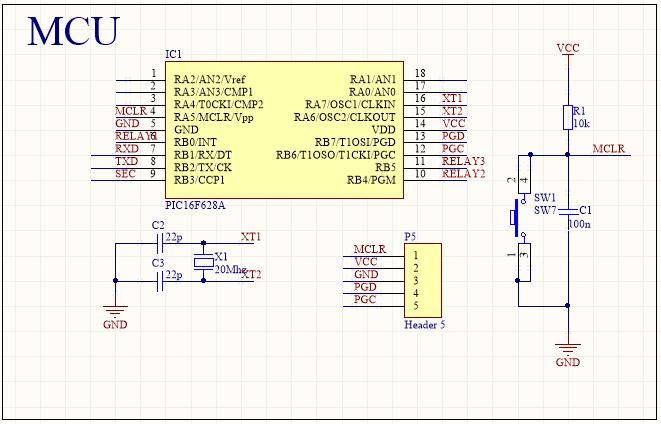
\includegraphics[scale=0.8]{images/mcuRelay.png}
    \caption{MCU of Slave Relay(s)}
    \label{fig:mcuRelay}
    \end{center}
\end{figure}

  \subsection{Button Block of Slave Button(s)} 
  \begin{figure}[!ht]
    \begin{center}
    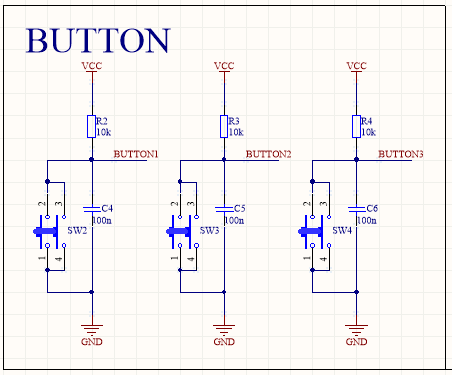
\includegraphics[scale=1]{images/button.png}
    \caption{Button block of Slave Button(s)}
    \label{fig:buttonBlock}
    \end{center}
  \end{figure}
  Figure~\ref{fig:buttonBlock} sketched the schematic of three-button block of Slave-3-Buttons, which means it is the typical block and may use for different numbers of buttons in one integrated circuit, depends on the decision of the author. In this thesis, the author used the same design for each button block, only increase or decrease the number of button if needed.

  \subsection{Relay block of Slave Relay(s)}
  \begin{figure}[!ht]
    \begin{center}
    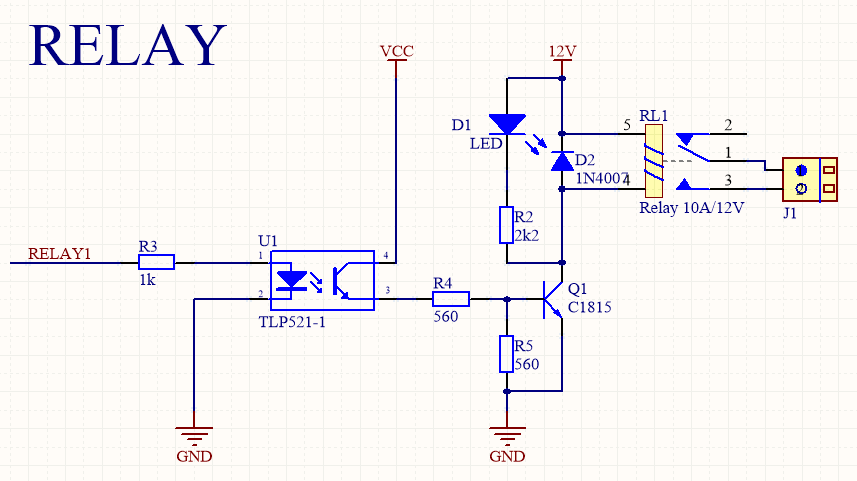
\includegraphics[scale=0.65]{images/relay.png}
    \caption{Relay block of Slave Relay(s)}
    \label{fig:relayBlock}
    \end{center}
  \end{figure}
  Relay is an electrical component which operates as a switch under electromagnetic working principle. It is useful when users need to switch state to control one to many circuit under one signal. A relay has two states are On and Off, switching bases on the current flows through its coil. Relay with parameters of 5 pins and 12V-10A DC is chosen in this thesis to ensure the switching circuit will operate accurately through long distance cable. Similar to Button block of Slave Button(s), the author use one design of a relay block and then increase or decrease the number of block in case needed. Figure~\ref{fig:relayBlock} shows one relay block of one of the Slave Relay(s) in the project.

\section{Security Camera Block}
When mention a security camera a few years back, people only think about an expensive system that only company level may afford and the system is massive itself, which make its mobility extremely low. However, world is changing rapidly, and with a household level, people still can implement a security camera system without paying a huge price but still, be provided with acceptable quality and performance. Furthermore, end users not only can view the security camera in fixed place but also can view camera from anywhere with Internet connection, an embedded computer and a device can connect to the Internet. In this thesis, the author built two function for Security Camera Block, which are Facial Recognition and Motion Detection. The first function is embedded onto a Mini Computer named Raspberry Pi 3, please see Figure~\ref{fig:rpiImage}, and second function, which is limited by resources from the author, will be integrated directly into Web Server as a prototype only.
\begin{figure}[!ht]
  \begin{center}
  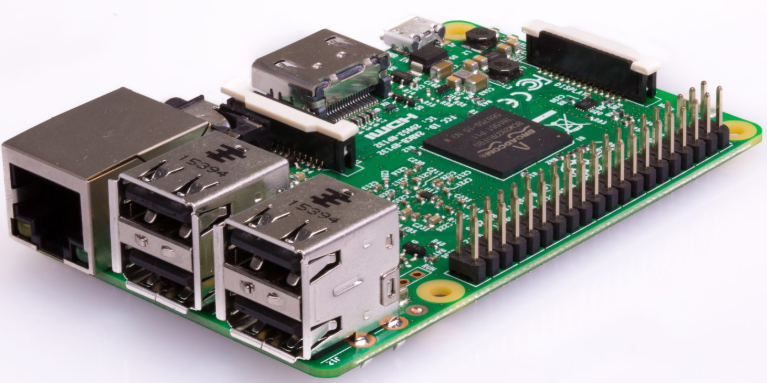
\includegraphics[scale=0.72]{images/rpi.png}
  \caption{Raspberry Pi 3 Model B}
  \label{fig:rpiImage}
  \end{center}
\end{figure}

Raspberry Pi 3 has market share at third place only followed by Mac and Windows. It is a mini computer, which means it has small size but has been integrated with every component that makes it a computer can in an ATM card size. Raspberry Pi 3 is the most powerful option of Pi series, but it has reasonable price with widely support documents and community because its operating system is Linux or Windows 10 IoT.  Also, with the supports from the operating system itself and the specifications listed as following, it is a suitable computer for this project. Besides, instead of using an USB camera through USB port, which also compatible with other types of computers, the author used camera modules that attached directly onboard of Raspberry Pi through CSI as in Figure~\ref{fig:piCamModule}. The significant advantage of the camera module compare to other USB camera is the huge different of quality of camera input stream and processing speed because it is built for Raspberry Pi. Please see Table~\ref{table:piCamSpecs} for few highlight specifications of Pi Camera Module. After connecting Pi Camera Module with Raspberry Pi 3 through CSI port via ribbon cable, Raspberry Pi should have the ability to view, record video, connect with and control the system via Wi-Fi connection after some configurations in next chapter of this thesis. Figure~\ref{fig:piAndCam} shows the standalone Raspberry Pi with Pi Camera Module attached. Furthermore, in the event that the owner need to add people into their recognition database, they can do it directly with Raspberry Pi and its PiCamera Module.

Raspberry Pi 3 Specifications:
\begin{itemize}
  \item SoC: Broadcom BCM2837.
  \item CPU: 4 core ARM Cortex-A53, clock 1.2GHz.
  \item GPU: Broadcom VideoCore IV.
  \item RAM: 1GB, bus 900Mhz.
  \item Connection: 10/100 Ethernet, 2.4GHz 802.11n, Bluetooth 4.1 Classic, BLE.
  \item GPIO: 40 pin.
  \item Others: 4x USB port, microSD, camera module port, HDMI.
\end{itemize}
\begin{figure}[!ht]
  \begin{center}
  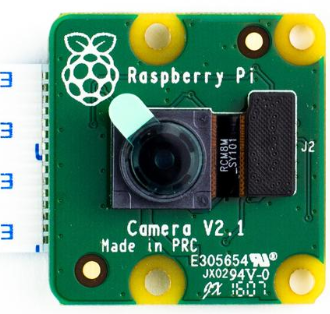
\includegraphics[scale=1]{images/piCamModule.png}
  \caption{Raspberry Pi Camera Module}
  \label{fig:piCamModule}
  \end{center}
\end{figure}
\begin{table}[h!]
  \begin{center}
  \begin{tabular}{ |c|c|  }
    \hline
    Attribute & Detail\\
    \hline
    Weight& 3g\\
    \hline
    Resolution&   8 Megapixels\\
    \hline
    Video modes &1080p30, 720p60 and 640 x 480p60,90\\
    \hline
    Linux integration & V4L2 driver available\\
    \hline
    Sensor resolution & 3280 x 2464 pixels\\
    \hline
    Sensor image area & 3.68 x 2.76 mm (4.6 mm diagonal)\\
    \hline
   \end{tabular}
   \caption{PiCamera Module Highlight Specifications}
   \label{table:piCamSpecs}
  \end{center}
  \end{table}
  \begin{figure}[!ht]
    \begin{center}
    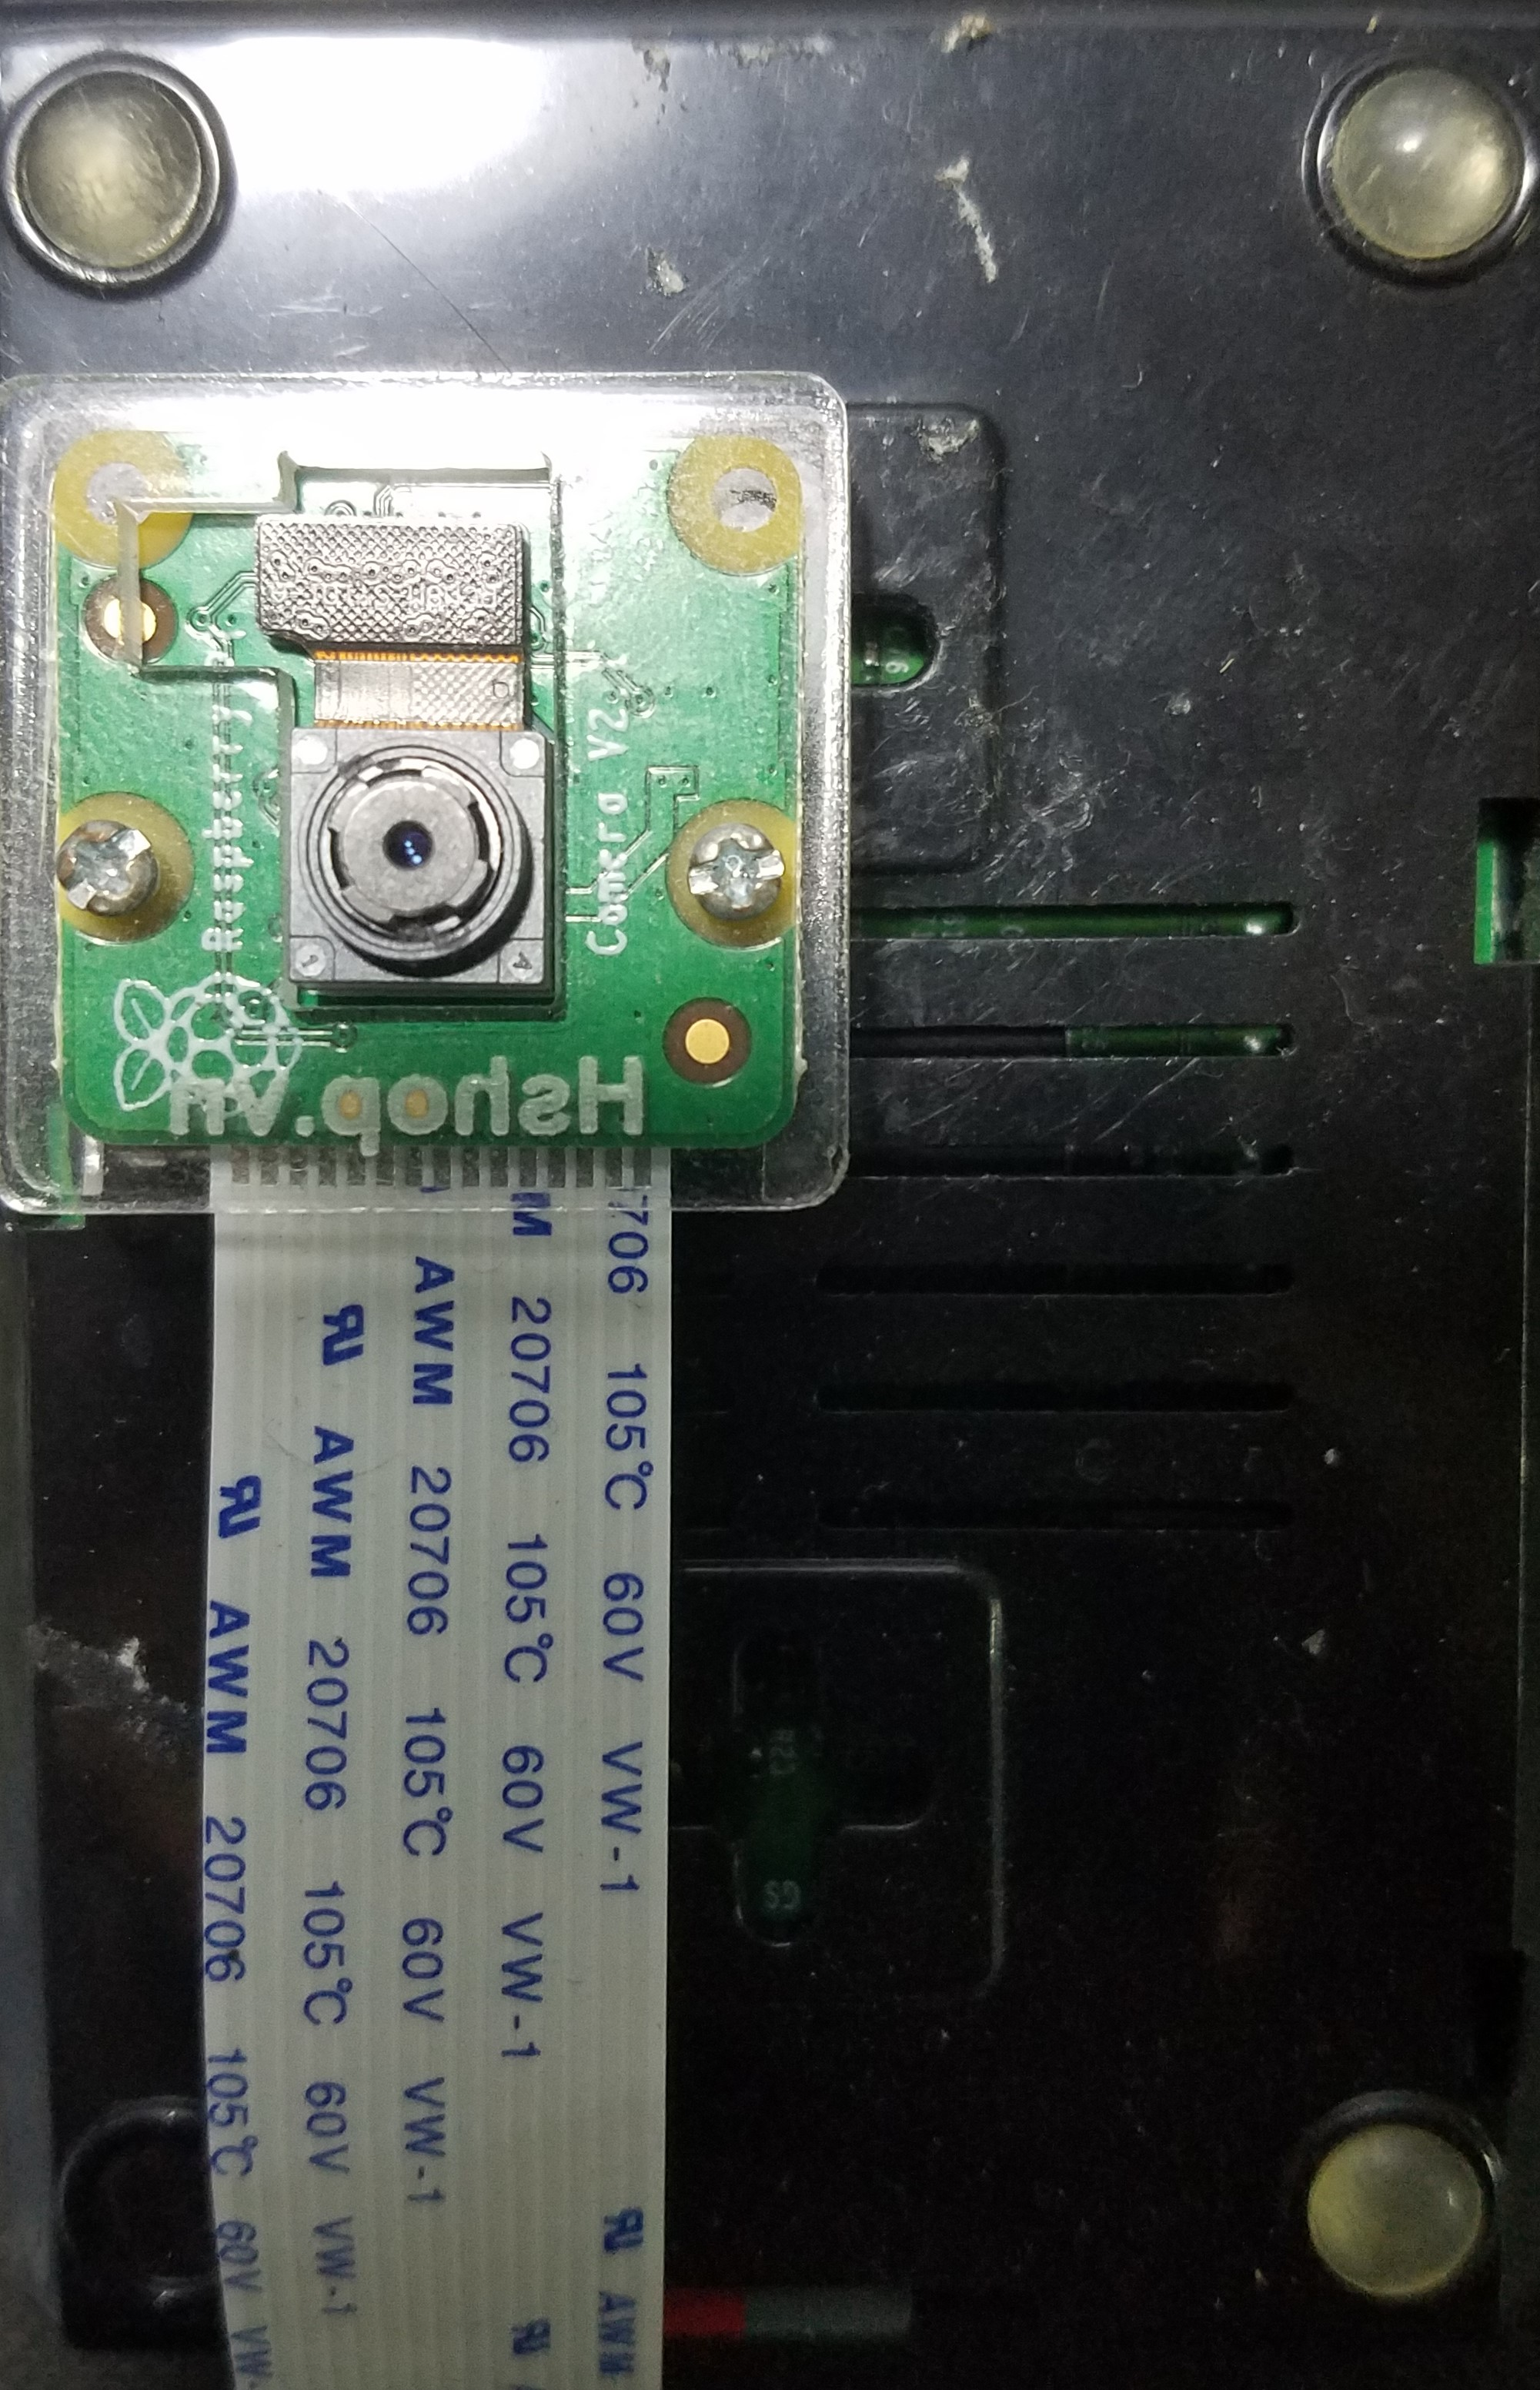
\includegraphics[scale=0.15]{images/piAndCam.jpg}
    \caption{Raspberry Pi Connected with PiCamera Module}
    \label{fig:piAndCam}
    \end{center}
  \end{figure}


\section{Full Schematic of the System}
Following are the full schematics of the system, namely Power for Master, Master, Slave button(s) and Slave Relay(s), respectively. The other modules which are not mentioned in section \ref{masterDesign} are the parts that may be extended in the future.
\begin{figure}[!ht]
  \begin{center}
  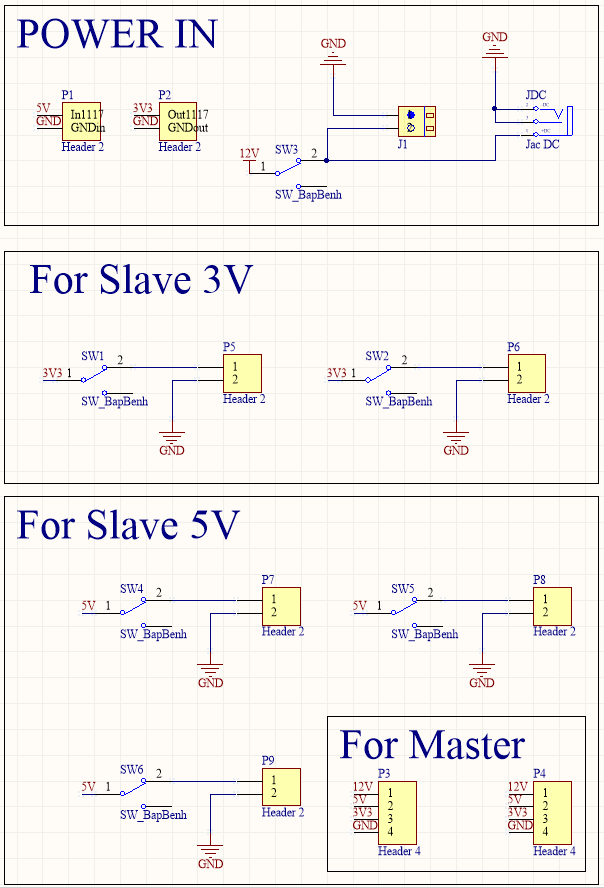
\includegraphics[scale=0.8]{images/powerMasterFull.PNG}
  \caption{Full Schematic of Power for Master}
  \label{fig:powerMasterFull}
  \end{center}
\end{figure}
\begin{figure}[!ht]
  \begin{center}
  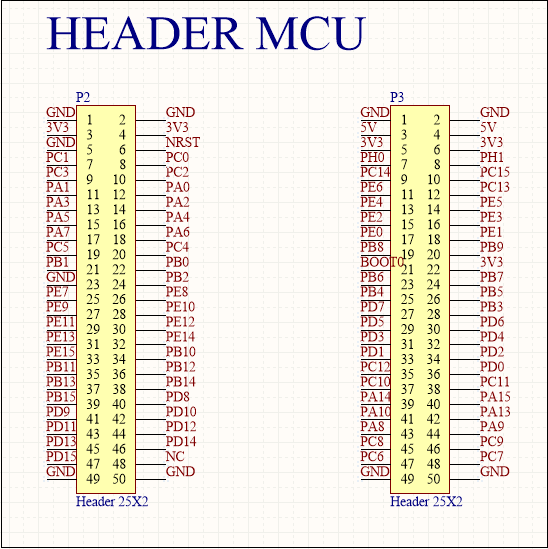
\includegraphics[scale=0.8]{images/headerMcu.PNG}
  \caption{Header for STM32F4 Discovery Kit}
  \label{fig:headerMcuFull}
  \end{center}
\end{figure}
\begin{figure}[!ht]
  \begin{center}
  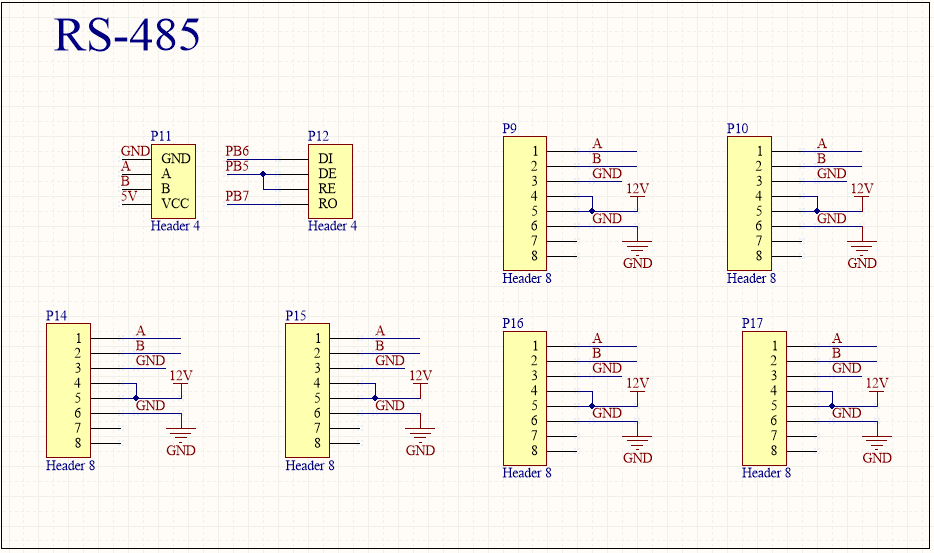
\includegraphics[scale=0.6]{images/header485.PNG}
  \caption{Master: Header for module RS-485 of Master}
  \label{fig:header485Full}
  \end{center}
\end{figure}
\begin{figure}[!ht]
  \begin{center}
  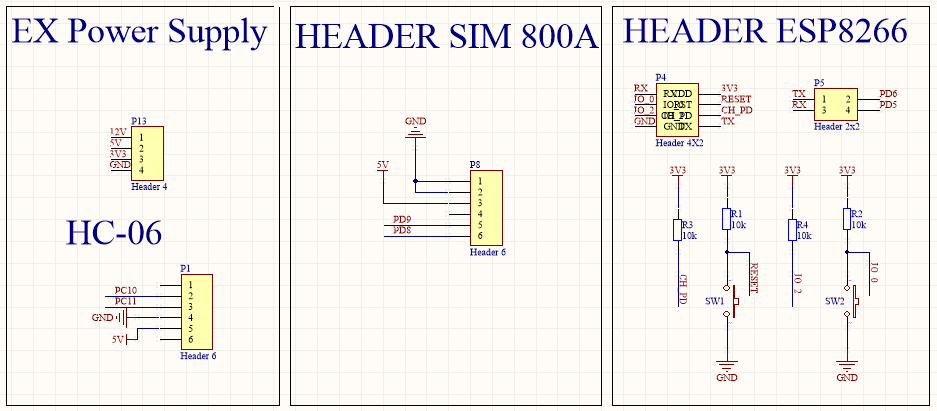
\includegraphics[scale=0.7]{images/masterLeft.PNG}
  \caption{Master: Header for other modules}
  \label{fig:masterLeftFull}
  \end{center}
\end{figure}
\begin{figure}[!ht]
  \begin{center}
  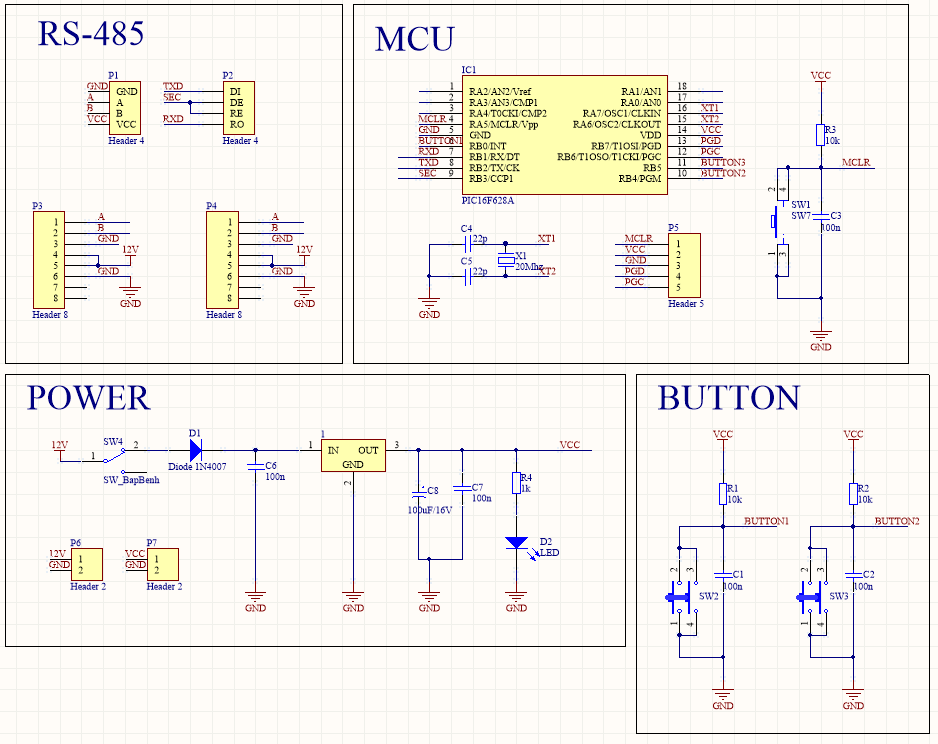
\includegraphics[scale=0.7]{images/slaveButtonFull.PNG}
  \caption{Slave Button(s)}
  \label{fig:slaveButtonFull}
  \end{center}
\end{figure}
\begin{figure}[!htbp]
  \begin{center}
  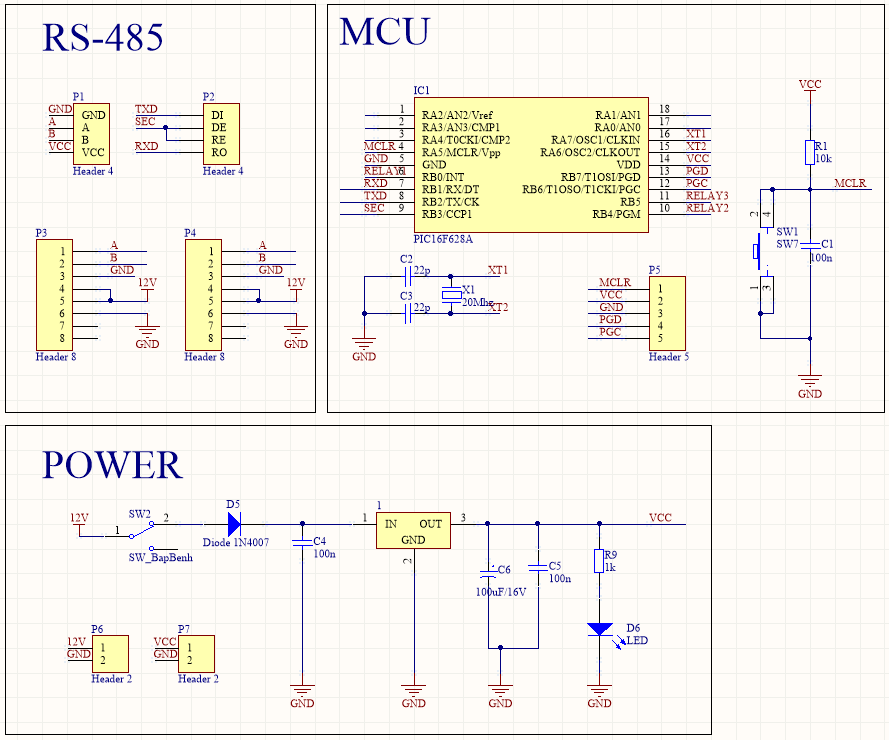
\includegraphics[scale=0.7]{images/slaveRelayFull1.PNG}
  \caption{Slave Relay(1)}
  \label{fig:slaveRelayFull1}
  \end{center}
\end{figure}
\begin{figure}[!ht]
  \begin{center}
  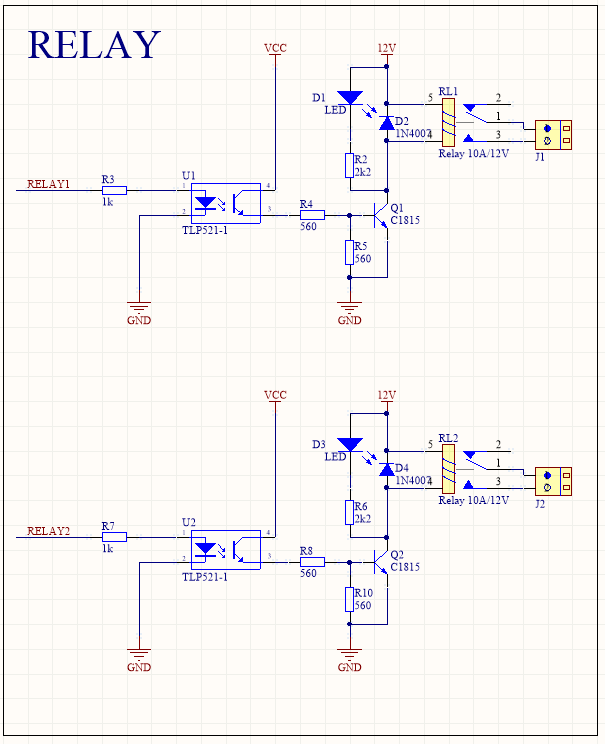
\includegraphics[scale=1]{images/slaveRelayFull2.PNG}
  \caption{Slave Relay(2)}
  \label{fig:slaveRelayFull2}
  \end{center}
\end{figure}